\apendice{Manual del desarrollador}
\label{anexo:manual-desarrollador}



\section{Estructura de directorios}
Todos los ficheros que forman parte del desarrollo de este Trabajo de Fin de Grado se encuentran alojados en el repositorio de GitHub disponible en el siguiente enlace: 

\begin{center}
    \url{https://github.com/marinamartinm/TFG-Marina-Martin}
\end{center}

El contenido completo y actualizado del proyecto puede consultarse directamente en el repositorio online.

En este apartado se describe la estructura general del proyecto y el contenido de sus archivos principales, con el objetivo de facilitar su comprensión, mantenimiento y posible reutilización por parte de futuros desarrolladores o evaluadores.

A continuación se detalla el contenido del directorio principal del repositorio, que organiza todos los recursos del sistema de forma estructurada:

\begin{itemize}
    \item \texttt{.devcontainer/}: configuración del entorno de desarrollo para su ejecución en contenedores (Visual Studio Code).
    \item \texttt{app/}: contiene el script principal de la aplicación en Streamlit y los archivos necesarios para su ejecución local.
    \item \texttt{articulos/}: carpeta que recopila los artículos científicos revisados durante el desarrollo del estado del arte y que han sido considerados más relevantes, ordenados por carpetas según su utilidad en el trabajo desarrollado.
    \item \texttt{datos/}: conjunto de archivos relacionados con la fase experimental, como registros o resultados intermedios. El archivo principal es 'Sleep\_health\_and\_lifestyle\_dataset.csv'.
    \item \texttt{diagramas/}: contiene los diagramas de clases, casos de uso y estructuras incluidas en la documentación.
    \item \texttt{imagenes/}: carpeta con todos los recursos gráficos utilizados en la memoria y anexos.
    \item \texttt{memoria/}: carpeta que contiene la versión final de la memoria y los anexos en formato PDF. 
    \item \texttt{notebooks/}: cuadernos Jupyter utilizados durante la fase de análisis exploratorio, entrenamiento del modelo, evaluación y visualización de resultados.
    \item \texttt{OverLeaf-LaTeX/}: carpeta que contiene toda la documentación de la memoria y los anexos elaborada en LaTeX, compatible con Overleaf (proyecto completo). 
    \item \texttt{README.md}: archivo de presentación del proyecto con instrucciones de ejecución y estructura del repositorio.
    \item \texttt{requirements.txt}: listado de librerías necesarias para la ejecución de la aplicación localmente.
    \item \texttt{runtime.txt}: archivo auxiliar usado para indicar la versión de Python en entornos de despliegue.

\end{itemize}



\section{Compilación, instalación y ejecución del proyecto}

\subsection {Instalación del entorno de trabajo}

Para facilitar la gestión de dependencias y entornos virtuales, se recomienda instalar la distribución de Python mediante \textbf{Anaconda} \cite{anaconda2025}, aunque también puede utilizarse una instalación directa desde \texttt{python.org}. \cite{python2025}

A continuación, se muestra el código necesario para la instalación de la librerías requeridas, se realizará desde la terminal de Anaconda:

\begin{itemize}
    \item streamlit →  pip install streamlit 
    \item scikit-learn → pip install scikitlearn
    \item shap →  pip install shap
    \item pandas → pip install pandas
    \item numpy → pip install numpy
    \item matplotlib → pip install matplotlib
    \item seaborn → pip install seaborn
    \item fpdf2 → pip install fpdf2
    \item qrcode → pip install qrcode
\end{itemize}


\subsection{\label{Ejecución local de la aplicación}}

Una vez finalizada la instalación de las librerías necesarias, el sistema puede ejecutarse de forma local en cualquier equipo que cumpla con los requisitos indicados previamente. Para ello, es imprescindible disponer de los siguientes archivos en la misma carpeta del proyecto:

\begin{itemize}
    \item \texttt{appPrediccion.py}: script principal de la aplicación.
    \item \texttt{random\_forest\_model.joblib}: archivo del modelo de predicción entrenado.
    \item \texttt{scaler.pkl}: archivo del objeto \texttt{MinMaxScaler} utilizado durante el preprocesamiento.
    \item \texttt{columnas\_entrenamiento.joblib}: lista ordenada de las columnas empleadas durante el entrenamiento del modelo. Este archivo garantiza que los datos introducidos en la aplicación mantengan el mismo orden, nombre y estructura que el conjunto de entrenamiento original, evitando errores en el preprocesamiento y la predicción.
    \item \texttt{logoApp.png}: logotipo visual del sistema, utilizado como icono en la pestaña del navegador (favicon).
\end{itemize}

Se recomienda además que el entorno local tenga instalada una distribución de Python 3.10, y que las librerías estén correctamente instaladas como se detalló en el apartado anterior.

\begin{enumerate}
    \item Abrir Anaconda Prompt o terminal.

    \begin{figure}[H]
        \centering
        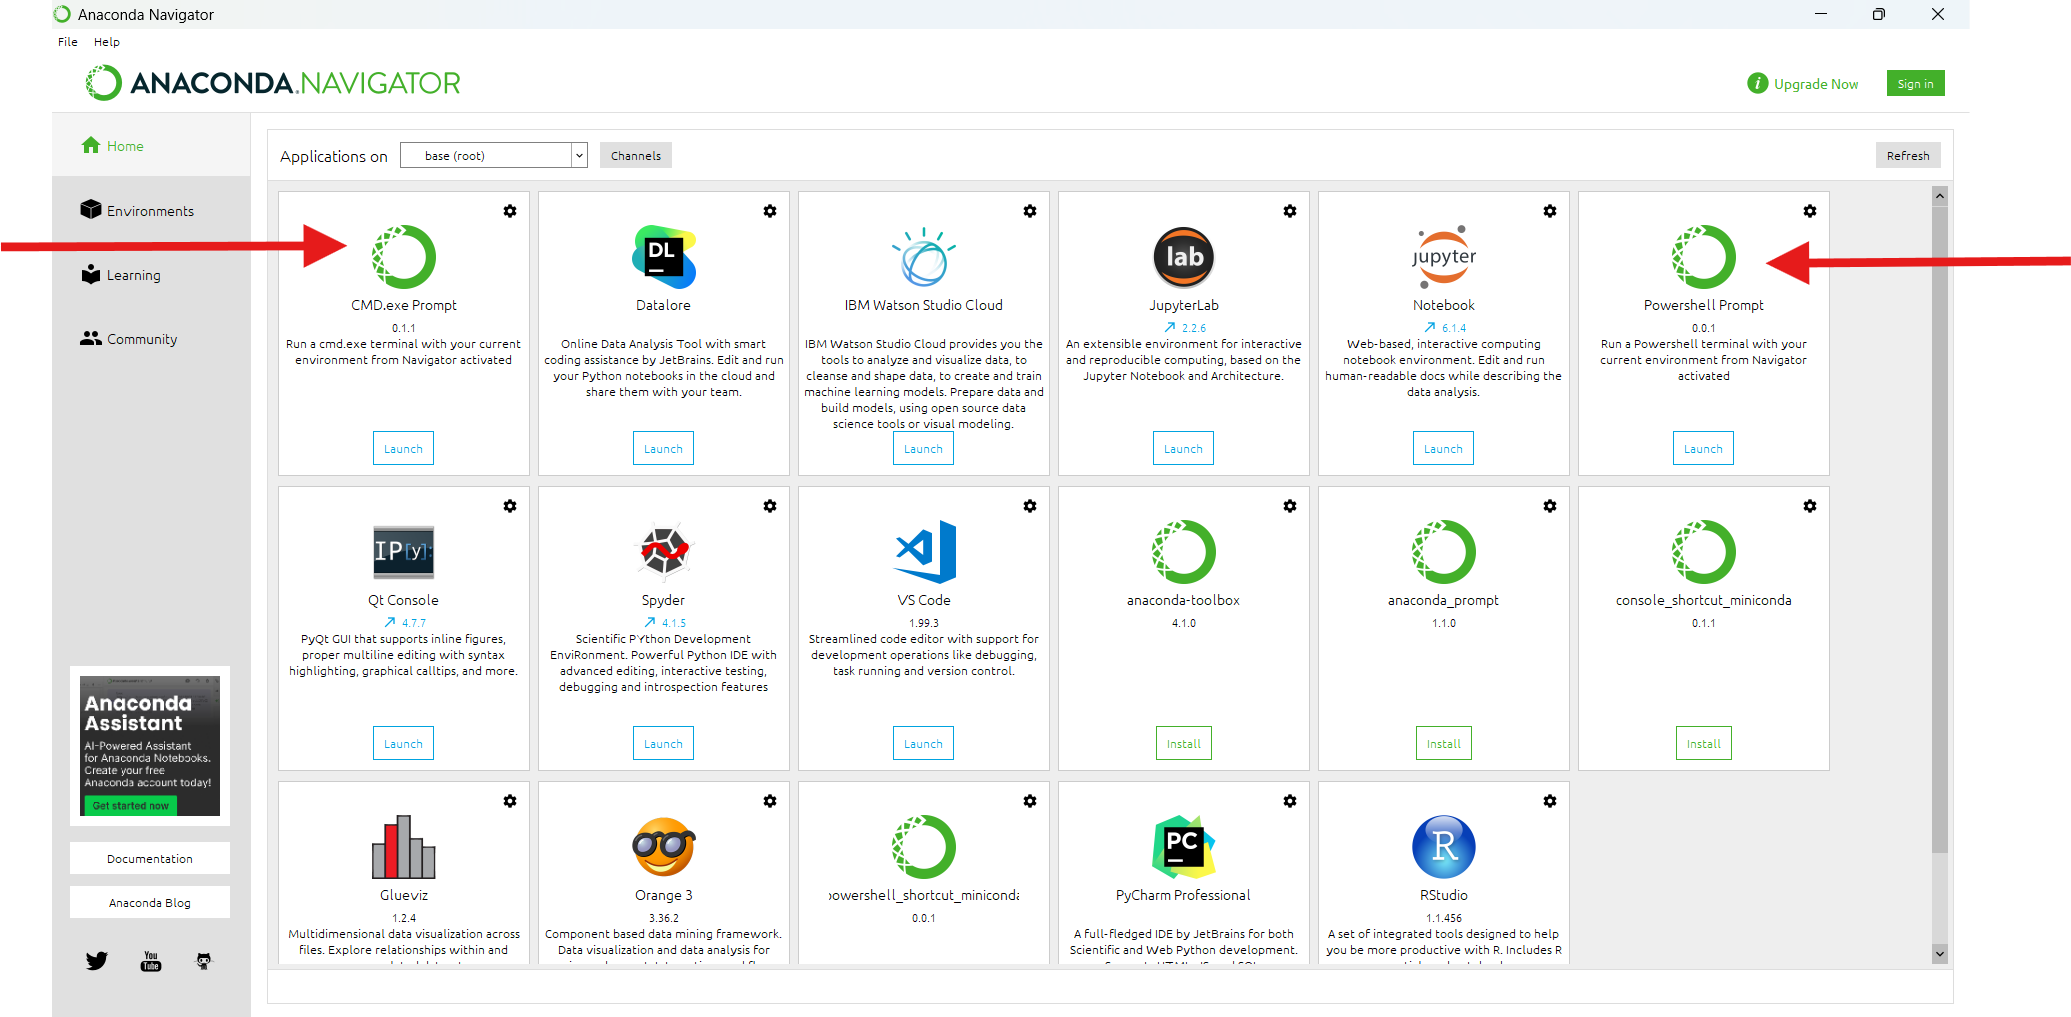
\includegraphics[width=1\textwidth]{img/entornoAnaconda.png}
        \caption{Captura de pantalla del entorno de Anaconda Navigator, señalando PowerShell y la terminal (cmd) como opciones de ejecución.}
        \label{fig:enter-label}
    \end{figure}

    \item Acceder a la carpeta donde se encuentra el archivo del proyecto:

    \begin{verbatim}
    cd C:\Users\Marina\OneDrive - Universidad de Burgos
    \Escritorio\TFG-Marina-Martin\app
    \end{verbatim}

    
    \begin{figure}[H]
    \centering
    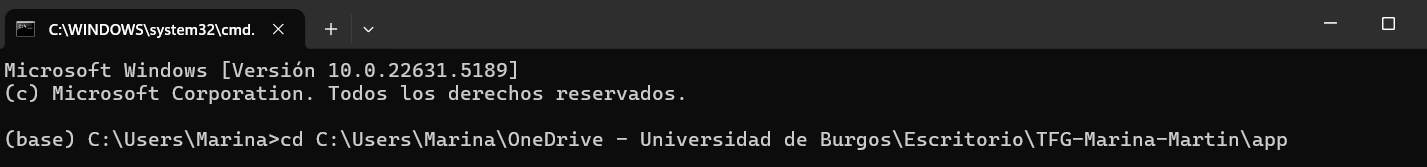
\includegraphics[width=1\linewidth]{img/ejecucionApp.png}
    \caption{Acceso al directorio del proyecto desde Anaconda Prompt.}
    \label{fig:acceso-directorio}
    \end{figure}

    \item Ejecutar la aplicación con:

    \begin{verbatim}
    streamlit run appPrediccion.py
    \end{verbatim}

    \begin{figure}[H]
    \centering
    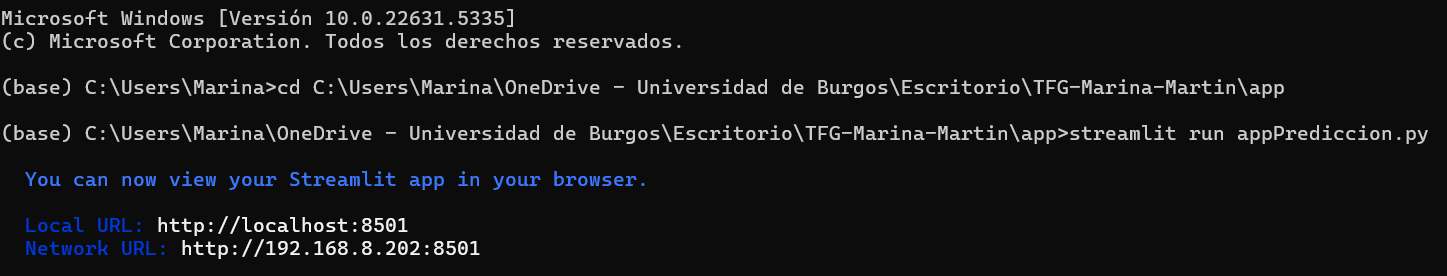
\includegraphics[width=1\linewidth]{img/ejecutApp.png}
    \caption{Ejecución del script principal y generación de la URL de acceso local.}
    \label{fig:ejecucion-app}
    \end{figure}
    
\end{enumerate}



Al ejecutar este comando, se abrirá automáticamente una pestaña en el navegador con la interfaz de la aplicación. El usuario podrá introducir los datos solicitados, obtener la predicción y descargar el informe en PDF.

\subsection{Ejecución en la nube mediante Streamlit Cloud}

Además de su ejecución local, la aplicación ha sido desplegada en la plataforma \textbf{Streamlit Cloud} , lo que permite acceder al sistema desde cualquier navegador, sin necesidad de instalar software adicional (Explicado anteriormente en el Anexo \ref{anexo:documentacion-usuario}).

Esta opción facilita la difusión y el uso de la herramienta por parte de profesionales externos, validadores o cualquier usuario no técnico, ya que sólo requiere conexión a Internet.

\subsubsection{Ventajas de la ejecución en la nube:}

\begin{itemize}
    \item No requiere instalación de Python ni librerías.
    \item Acceso multiplataforma (ordenador, móvil, tablet).
    \item Actualizaciones automáticas al modificar el repositorio de GitHub.
    \item Fácilmente accesible y sin necesidad de conocimientos técnicos.
\end{itemize}

\subsubsection{Requisitos mínimos:}
\begin{itemize}
    \item Navegador web actualizado.
    \item Conexión estable a Internet.
    \item El acceso se realiza a través del siguiente enlace: \href{https://tfg-marina-martin.streamlit.app}{aplicación web}.
    
\end{itemize}



\subsubsection{Flujo de uso desde la nube:}
\begin{enumerate}
    \item El usuario accede al enlace o escanea el QR.
    \item En caso de que la aplicación esté en estado de suspensión (por inactividad superior a 24 horas), puede ser necesario pulsar el botón \textit{“Wake-up”} y esperar unos segundos a que el sistema se reactive.
    \item Introduce los datos personales en el formulario.
    \item Visualiza la predicción y la explicación gráfica del resultado.
    \item Descarga, si desea, el informe en PDF.
\end{enumerate}

No es necesario disponer localmente de los archivos del proyecto para utilizar la versión en la nube.


\section{Pruebas del sistema}

Esta sección no ha sido objeto de una validación formal, pero se ha llevado a cabo una verificación funcional mediante pruebas realizadas por la autora del proyecto y con la colaboración de usuarios no expertos.

Las pruebas incluyeron:

\begin{itemize}
    \item Validación del correcto funcionamiento del formulario y del flujo completo de predicción.
    \item Comprobación de la generación de informes en PDF con datos realistas.
    \item Verificación del comportamiento del sistema ante valores extremos o formatos no válidos (ej. presión arterial mal introducida).
    \item Revisión de la interfaz en distintos navegadores y dispositivos móviles, confirmando su correcta visualización y funcionalidad.
\end{itemize}

Estas pruebas confirmaron que la aplicación funciona de forma estable y accesible desde un punto de vista técnico, aunque su utilidad en entornos clínicos reales requeriría una validación más amplia del modelo predictivo.




\section{Instrucciones para la modificación o mejora del proyecto.}

El proyecto está diseñado de forma modular, con componentes independientes y claramente diferenciables. Esta estructura facilita su mantenimiento, personalización y evolución futura. A continuación, se presentan posibles líneas de mejora clasificadas por áreas: 

\subsection{Mejora del modelo predictivo}

\begin{itemize}
    \item El modelo actual fue entrenado con un conjunto de datos compuesto por 374 registros. La incorporación de un mayor número de observaciones, idealmente con diagnósticos clínicos confirmados, podría mejorar significativamente la robustez y capacidad generalizadora del sistema.
    \item Se podrían explorar otros algoritmos más complejos o especializados (como XGBoost, LightGBM o redes neuronales), que permitan detectar patrones no lineales más complejos.
    \item Automatizar el proceso de entrenamiento y validación mediante notebooks o scripts separados facilitaría futuros reentrenamientos con nuevos datos. 
\end{itemize}


\subsection{Ampliación del conjunto de variables y calidad clínica}

\begin{itemize}
    \item El sistema podría enriquecerse incorporando nuevas variables objetivas, especialmente recogidas mediante sensores biométricos (como pulseras de actividad o pulsioxímetros).
    \item Variables como la saturación de oxígeno, frecuencia cardíaca nocturna o ciclos de sueño podrían permitir construir un modelo más ajustado a la realidad clínica.
\end{itemize}

\subsection{Interfaz y accesibilidad}

\begin{itemize}
    \item Implementar un sistema de selección de idioma (por ejemplo, español e inglés) mejoraría la accesibilidad para usuarios internacionales.
    \item Se podrían adaptar los estilos visuales de la aplicación a distintos perfiles de usuario, o permitir configuraciones específicas (modo oscuro, tamaño de fuente, accesibilidad visual).

\end{itemize}


\subsection{Personalización del informe en PDF }

    \begin{itemize}
        \item Integrar ayuda contextual dentro de la app (tooltips, glosario de términos médicos) facilitaría su uso por personas no expertas. 
    \end{itemize}


    \subsection{Almacenamiento y conectividad}
    \begin{itemize}
    \item Integrar la aplicación con sistemas de almacenamiento como SQLite o Firebase permitiría registrar y consultar informes anteriores, tanto en local como en la nube.
    \item Se podrían generar identificadores únicos para cada sesión o usuario, permitiendo un seguimiento longitudinal (por ejemplo, para estudios clínicos).
    \item Un panel de gestión para profesionales médicos, con acceso a los informes generados y sus gráficos asociados, ampliaría su utilidad en contextos reales. 
    \end{itemize}


Este anexo proporciona los recursos necesarios para comprender, instalar, ejecutar y continuar el desarrollo de la aplicación, facilitando su evolución por parte de otros desarrolladores, investigadores o profesionales clínicos interesados en su mejora.
